% !TeX root = ../../main.tex
\newpage
\section{Sieć \textit{Mask R-CNN}}

Sieć \textit{Mask R-CNN} \cite{matterport-mask-rcnn} jest otwartoźródłowym projektem wykorzystującym następujące technologie: \textit{Python3} \cite{python}, \textit{TensorFlow} \cite{tensorflow} oraz \textit{Keras} \cite{keras}. Konkretne wersje i dodatkowe zależności zawarte są w Dodatku A.

Główne komponenty, na które składa się dołączony program to:

\begin{itemize}
  \item plik \texttt{config.py}, zawierający konfigurację i hiperparametry modelu;
  \item plik \texttt{model.py}, odpowiadający za stworzenie modelu;
  \item plik \texttt{utils.py}, zawierający funkcje pomocnicze;
  \item skrypt \texttt{train.sh}, służący do trenowania sieci;
  \item skrypt \texttt{validate.sh}, umożliwiający badanie skuteczności metody.
\end{itemize}

\subsection*{Konfiguracja i hiperparametry modelu}

Konfiguracja i hiperparametry zawarte są w pliku \texttt{config.py}. Umożliwia on konfigurowanie m.in. następujących parametrów:
\begin{itemize}
  \item współczynnika uczenia (z ang. \textit{learning rate}) - parametr wpływający na szybkość uczenia; strategię doboru tego parametru opisano w Rozdziale \numberref{sec:hiperparametry};
  \item liczba wykorzystywanych kart graficznych - proces uczenia można przyspieszyć wykorzystując wiecej niż jedną kartę graficzną; w ramach niniejszej pracy wykorzystywano jedną kartę graficzną (\textit{GeForce GTX 1080} z 8GB dostępnej pamięci, użyczoną przez firmę \blue{});
  \item liczba klas (w przypadku niniejszej pracy są rozpoznawane dwie klasy, tzn. kort badmintona oraz brak kortu).
\end{itemize}

\subsection*{Klasy i funkcje do stworzenia modelu}
Klasy i funkcje służące do stworzenia modelu \textit{Mask R-CNN} zostały zawarte w pliku \texttt{model.py}. Umożliwiają one wytrenowanie modelu oraz pozwalają na detekcję obszaru kortu na podanych obrazach wejściowych. Klasa modelu pozwala zapisać wytrenowane wagi na dysku oraz wczytać wagi z pliku.

\subsection*{Funkcje pomocnicze}
Funkcje pomocnicze, które używane są w różnych miejscach w kodzie umieszczono w pliku \texttt{utils.py}.
Funkcje te realizują m.in:

\begin{itemize}
  \item wczytanie obrazów z dysku - obrazy w formacie \textit{JPG} lub \textit{PNG} wczytywane są jako trójwymiarowa tablica liczb; wymiary obrazu to wysokość, szerokość oraz kanały koloru;
  \item wczytanie anotacji danych - anotacje zapisane są na dysku w formacie \textit{JSON}; oprócz wczytania obrazów, konieczne jest wczytanie odpowiadających im anotacji;
  \item zmiana rozdzielczości obrazu - pozwala zmienić rozdzielczość wczytanego obrazu do pożądnej rozdzielczości; sieć ma stałą liczbę neuronów w warstwie wejściowej, dlatego też stosuje się zmianę rozdzielczości, aby obraz mógł być użyty na wejściu tej warstwy;
  \item pobranie modelu wytrenowanego na zbiorze \textit{COCO} \cite{coco}.
\end{itemize}

\subsection*{Trenowanie sieci}

Trenowania sieci przy użyciu skryptu \texttt{train.sh} polega na uruchamieniu jednego lub więcej treningów, jeden po drugim. Taka seria treningów uruchamiana jest na podstawie zestawu plików opisujących dany trening, czyli precyzujących na jakim zbiorze danych ma zostać przeprowadzony trening, jaki powinien być podział na podzbiory treningowe i walidacyjne wybranego zbioru oraz czy trenować oryginalną implementację \textit{Mask R-CNN}, czy też wersję zmodyfikowaną. Skrypt posiada funkcjonalność powiadamiania za pomocą wysyłania poczty elektronicznej - wiadomość wysyłana jest po każdym zakończonym treningu z informacją, czy trening zakończył się sukcecem lub czy wystąpił błąd.

\subsection*{Skuteczność metody}

Badanie skuteczności metody przeprowadzono przy użyciu skrypty \texttt{validate.sh}, który operuje na rezultatach skryptu \texttt{train.sh} trenującego sieć.
Dla każdego przeprowadzonego treningu, uruchamiany jest wytrenowany model i sprawdzane jest jego działanie na podzbiorach walidacyjnych i testowych zbioru \textit{low} i \textit{high}. Na podstawie wyników na zbiorze walidacyjnym, wyliczane są wyniki opisane w~Rozdziale \myrefx{sec:miary}, natomiast wyniki sieci na podzbiorze testowym są zapisywane na dysku jako bazowy obraz z nałożoną przezroczystą maską przewidzianego kortu, na potrzeby ręcznej weryfikacji skuteczności. Przykład takiego testowego obrazu
ze zbioru \textit{high} przedstawiono na Rysunku \numberref{fig:testexample}.


Wynikiem weryfikacji modelu na zbiorze walidacyjnym jest tablica pomyłek. Na podstawie anotacji danych i maski detektowanego obszaru kortu, dla każdego rekordu zbioru walidacyjnego, zapisywana jest liczba pikseli zaklasyfikowanych jako przypadek prawdziwie pozytywny, prawdziwie negatywny, fałszywie pozytywny i fałszywie negatywny. Na podstawie tych liczb obliczane są miary dokładności, swoistości, czułości i~precyzji opisane w~Rozdziale \myrefx{sec:miary}. Na koniec dla poszczególnych miar obliczana jest średnia, mediana, minimum oraz maksimum.

\begin{figure}[!htb]
  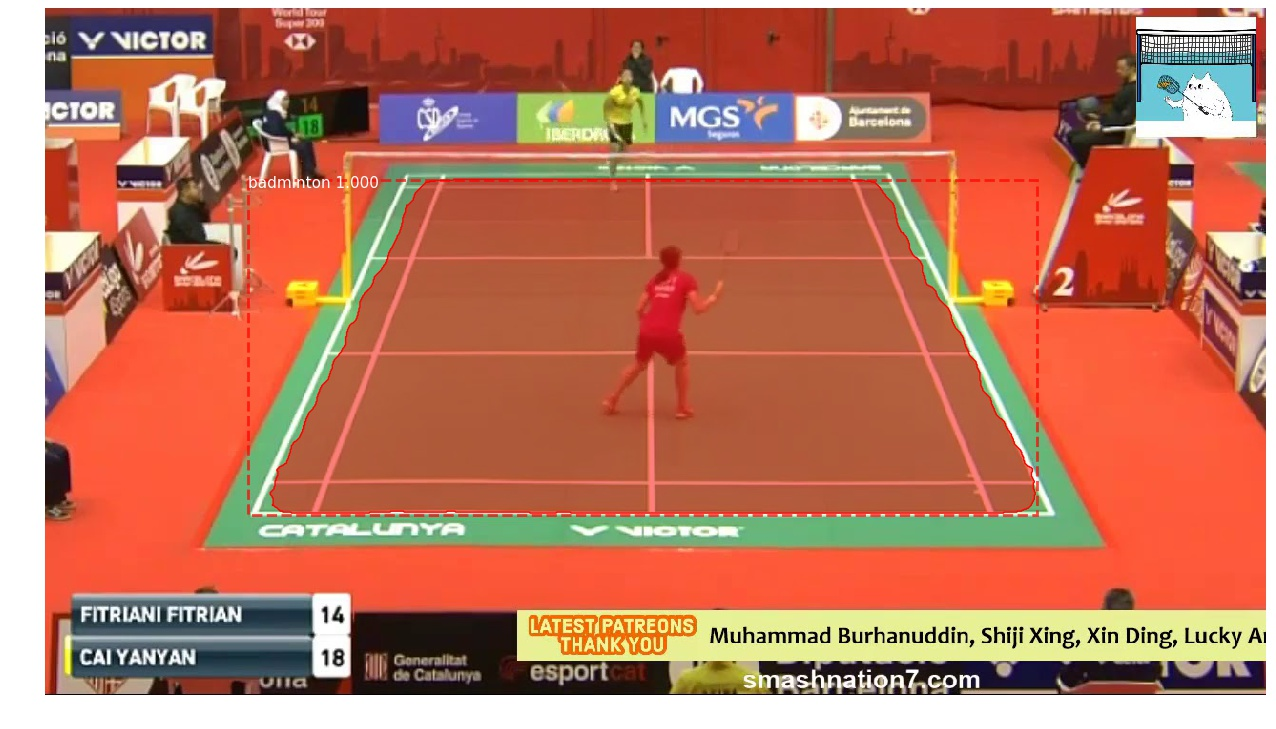
\includegraphics[width=\linewidth]{./ss2.jpg}
    \caption{Przykład obrazu testowego ze zbioru \textit{high} z nałożoną maską detektowanego obszaru kortu}
    \label{fig:testexample}
\end{figure}
